\documentclass[twocolumn]{article}
\usepackage[letterpaper, margin=1in]{geometry}
\usepackage{parskip}
\usepackage{fancybox}
\usepackage[table]{xcolor}
\usepackage{amsmath}
\usepackage{graphicx}
\usepackage[most]{tcolorbox}

\usepackage{adjustbox}
\usepackage{titling}
\title{Project 2: K-Means Strategy}
\author{Youmi Koh}
\date{Sep 16, 2023}

\makeatletter
\def\@maketitle{
\newpage
 \null
 \vskip 0em
 \begin{center}
  {\LARGE \@title \par}%
  {\large \@author \par}%
  {\large \@date \par}%
 \end{center}%
 \vskip 1.8em}
\makeatother

\usepackage{fancyhdr}
\fancypagestyle{plain}{
    \fancyhf{}
    \fancyhead[L]{CSE575 - Fall 2023}
    \fancyhead[R]{Student ID: 1231025486}
}

\makeatletter
\renewcommand{\verbatim@font}{\scriptsize\ttfamily}
\makeatother

\begin{document}
\maketitle
\noindent

This project highlights k-means in the context of different strategies for selecting the initial cluster centers. K-means is applied to a dataset of 2-D points, and the following objective function is used to evaluate performance:
\[
    \begin{array}{lll}
        \operatorname{argmin}_{C,\mu} \sum\limits_{i=1}^{k}\sum\limits_{x\in C_i}||x-\mu_i||^2 & \text{where} & \textstyle k\ \text{clusters, } C_i\ \text{i\textsuperscript{th}} \text{ cluster, } \mu_i\ \text{mean of } C_i
    \end{array}
\]

\subsubsection*{Strategy 1: Randomly select the initial cluster centers}

\begin{minipage}[t]{1\textwidth}
    \begin{minipage}[h]{9cm}
        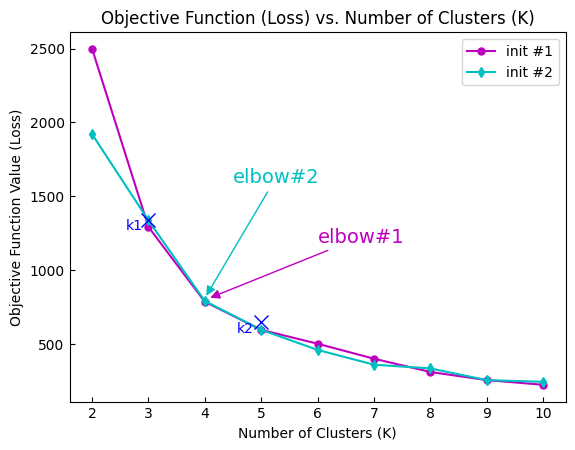
\includegraphics[width=1\textwidth]{strategy1output.png}
    \end{minipage}
    \begin{tabular}[p]{|p{3.5cm}p{3.5cm}|}
        \hline
        \begin{minipage}[t]{3.5cm}
            \begin{verbatim}
k1=3
k1_loss=1338.1076016520997
k1_initial_centers=[
    [4.95185958 4.11756694]
    [2.44868927 2.55261552]
    [3.02105687 9.26213796]
k1_final_centroids=[
    [7.23975119 2.48208269]
    [3.23489005 2.5530322 ]
    [4.83091958 7.29959959]]\end{verbatim}
            \vspace{0.3\baselineskip}
        \end{minipage}
         & \begin{minipage}[t]{3.5cm}
               \begin{verbatim}
k2=5
k2_loss=649.9266570480959
k2_initial_centers=[
    [4.34489155 3.99726667]
    [2.47238755 3.7285616 ]
    [2.80096609 1.03176348]
    [7.30246332 3.16580577]
    [3.98724311 4.0425478 ]]
k2_final_centroids=[
    [6.60345839 7.57042104]
    [3.49556658 3.56611232]
    [3.14506148 0.90770655]
    [7.41419243 2.32169114]
    [2.81706606 7.010913  ]]\end{verbatim}
               \vspace{0.3\baselineskip}
           \end{minipage} \\ \hline
    \end{tabular}
\end{minipage}


The consistency and quality of the initial centers are can vary when using a random selection strategy. As highlighted in the \textit{Loss vs. K} graph graph above, losses can differ significantly despite having the same number clusters, as shown in the $k=2$ instance. A poor starting center selection can lead to K-means converging to local optima centroid with suboptimal clusters. In the \textit{Local Optima Centroid} graph below, we can see that initialization \#1 gets stuck in a local optima and the final centroids are not well positioned. This results in a higher loss than that of initialization \#2, which converges to a superior centroids. One method of overcoming this sensitivity to initial centers is running multiple initialization and selecting the best results.

As expected, the loss decreases as the number of clusters increases. The rate of improvement slows down as the number of clusters increases. This is because the marginal improvement of adding a new cluster is smaller than the marginal improvement of adding the previous cluster. The optimal number of clusters is the point where the marginal improvement is no longer significant. In this case, the elbow point depicts the kink where the previously steep improvements are plateauing. In the above graph, the elbow point is at $k=4$.

\newpage

\begin{figure}[t]
    \centering
    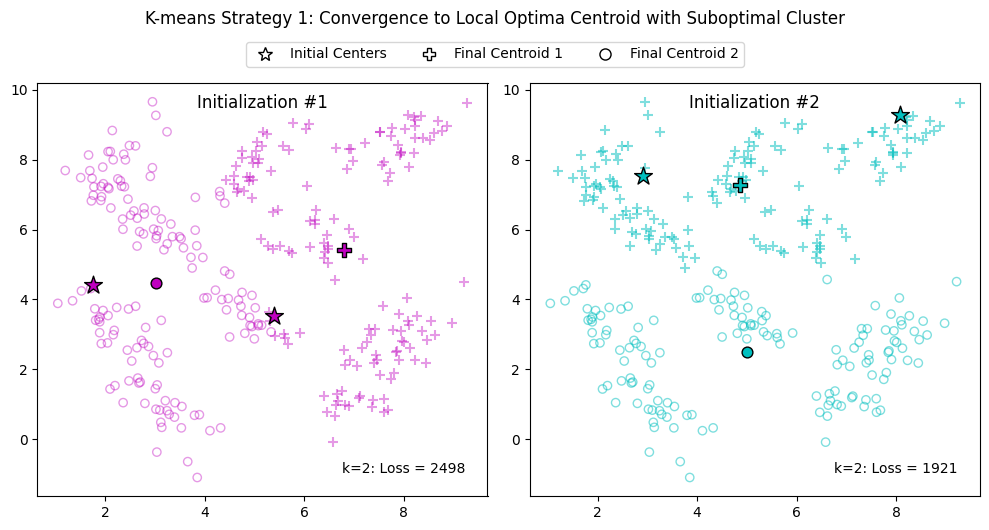
\includegraphics[width=0.8\textwidth]{cluster_output.png}
\end{figure}

\subsubsection*{Strategy 2: Select $i$th initial center to be max average distance from all preceding centers}

Deliberately selecting initial centers to be as distant as possible from each other produces more consistent starting states. It reduces the sensitivity to initial centroids as seen in Strategy 1, and yields more accurate clusters. With both strategies and in all 4 initializations, the resulting final centroids from K-means shows that the optimal $k$ is 4, as indicated by the elbow points below.

\begin{minipage}[t]{1\textwidth}
    \begin{minipage}[h]{8cm}
        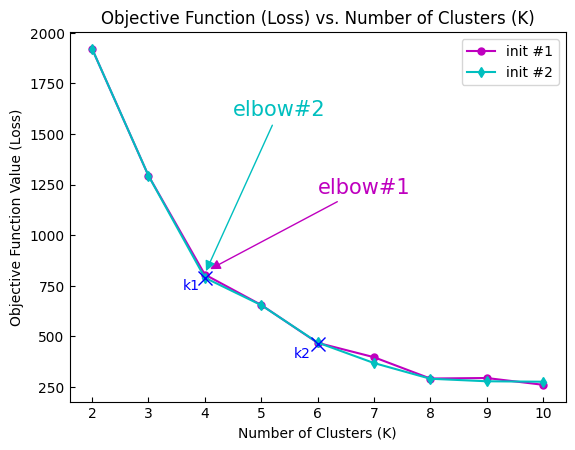
\includegraphics[width=1\textwidth]{strategy2output.png}
    \end{minipage}
    \begin{tabular}[p]{|p{4cm}|p{4cm}|}
        \hline
        \begin{minipage}[t]{4cm}
            \begin{verbatim}
k1=4
k1_initial_given=[
    2.5366924  2.24222672]
k1_loss=788.2693490065562
k1_initial_centers=[
    [2.5366924 , 2.24222672],
    [9.26998864, 9.62492869],
    [ 3.85212146, -1.08715226],
    [2.95297924, 9.65073899]]
k1_final_centroids=[
    [3.33995748 2.59215224]
    [6.60345839 7.57042104]
    [7.38076264 2.33245532]
    [2.85859235 6.93136525]]\end{verbatim}
            \vspace{0.3\baselineskip}
        \end{minipage}
         & \begin{minipage}[t]{4cm}
               \begin{verbatim}
k2=6
k2_initial_given=[
    4.5872861  7.29024049]
k2_loss=462.9263558248374
k2_initial_centers=[
    [4.5872861 , 7.29024049],
    [ 3.85212146, -1.08715226],
    [9.26998864, 9.62492869],
    [1.20162248, 7.68639714],
    [ 6.5807212, -0.0766824],
    [8.87578072, 8.96092361]]
k2_final_centroids=[
    [5.23053667 4.2793425 ]
    [2.68198633 2.09461587]
    [7.91430998 8.51990981]
    [2.54165252 7.00267832]
    [7.55616782 2.23516796]
    [5.24028296 7.53131029]]\end{verbatim}
               \vspace{0.3\baselineskip}
           \end{minipage} \\ \hline
    \end{tabular}
\end{minipage}


\end{document}
